\documentclass[sigconf]{acmart}
\setcopyright{none}
\settopmatter{printacmref=false,printfolios=true,authorsperrow=3}
\renewcommand\footnotetextcopyrightpermission[1]{}
\acmDOI{}\acmISBN{}\acmConference{}{}{}
\providecommand{\Description}[1]{}
\usepackage{booktabs}
\usepackage{listings}
\lstset{language=SQL,basicstyle=\ttfamily\scriptsize,breaklines=true,columns=fullflexible,keepspaces=true,showstringspaces=false,aboveskip=3pt,belowskip=3pt}
\newcommand{\repolink}{\url{https://github.com/harrishmarro/Retail-Mesh-Intelligence}}
\begin{document}
\title{Retail-Mesh Intelligence: A Relational Implementation}
\titlenote{Project repository: \repolink. The attached new ER package supersedes the older repository diagram.}
\author{Avlyn Kaur Khurana}
\affiliation{\institution{University of Victoria}\country{Canada}}
\author{Harish Pugazhenthi Sasikala}
\affiliation{\institution{University of Victoria}\country{Canada}}
\author{Krishnaswamy Gopalakrishnan}
\affiliation{\institution{University of Victoria}\country{Canada}}
\begin{abstract}
Retail-Mesh connects legal providers, vehicle activities, verified customer accounts, performance evidence and incentive entitlements. We map the newly supplied 26-entity ER model to 34 SQLite relations, preserving business identities alongside surrogate keys. A local web interface supports data entry, search, modification and deletion. Reproducible SQL demonstrates a sale--service--replacement-rental journey without merging source accounts or transferring a reward to an evidence contributor. Source and evaluation artifacts are prepared for \repolink; this local implementation has not been pushed. Author ordering and human evaluation remain team review items.
\end{abstract}
\keywords{relational modeling, SQLite, vehicle retail, identity evidence, reproducibility}
\maketitle
\pagestyle{plain}\fancyhead{}
\section{Domain and Information Needs}
A vehicle can be sold by Dealer A, serviced by Provider C, and supported by a replacement rental from Provider B. Flat customer and vehicle lists obscure which legal provider performed each activity, whether customer accounts were verified as related, and which provider earned an incentive. Retail-Mesh records these distinctions. The relational milestone implements storage and querying; knowledge graphs, automated identity verification and a general incentive calculation engine remain future scope.

The authoritative input is the newly attached crow's-foot ER package, containing 26 entities and 42 named relationships. The older diagram in the repository is not a design input. Business identifiers are proposed source identities and require validation against real records; the demonstration uses entirely synthetic data.
\section{ER-to-Relational Mapping}
\subsection{Providers, Activities and Account Identity}
ParentCompany and Provider preserve jurisdiction and registration number as composite candidate keys. Outlet and CustomerAccount identities remain provider-scoped; source namespaces distinguish local account references. CustomerIdentityLink connects a canonical account pair and stores verification status, method and evidence. It does not invent a global customer identifier or imply transitive identity.

Vehicle references its catalogue model and preserves VIN uniqueness. VehicleActivity references its issuing outlet, local customer account and vehicle. Sale, Rental and Service each have their own autogenerated Id and a UNIQUE activity FK. Bidirectional deferred composite FKs and a kind CHECK enforce the total, disjoint specialization at transaction commit. The application inserts the parent and exactly one subtype atomically. Rental optionally references Service and records ReplacementPurpose, preserving the distinction between the serviced and replacement VINs.
\subsection{Policies, Evaluations and Entitlements}
ProgramEnrollment and provider/capability authorizations retain dated associations. RuleVersion and MetricDefinitionVersion preserve effective definitions. PerformanceMeasurement has provider--definition--period grain. MeasurementContribution and RuleMetric resolve two many-to-many relationships. Six further associative relations preserve event/period measurement, activity and identity evidence, including relationship attributes.

EventEvaluation has activity--rule-version grain; PeriodEvaluation adds provider and period. Stable awards use the unversioned rule and subject identity, preventing duplicate entitlements across policy versions. Each award references a qualified, matching evaluation and at least one owned benefit component. Currency, unit scheme and unit code remain explicit; cash and points are never summed together.

All 34 relations have an autogenerated integer \texttt{Id}; displayed business keys are also mandatory UNIQUE constraints. FK enforcement is enabled per connection. Referenced records cannot be deleted while dependents remain. Dates and UTC timestamps, nonnegative benefits, canonical identity pairs, nonoverlapping effective intervals and qualification-date version applicability are checked. Final evaluations and cited source evidence are immutable; accepted evidence cannot be appended or rewritten. Current identity assertions may later be revoked without altering stored decision snapshots.

\clearpage
\begin{figure}[t]
\centering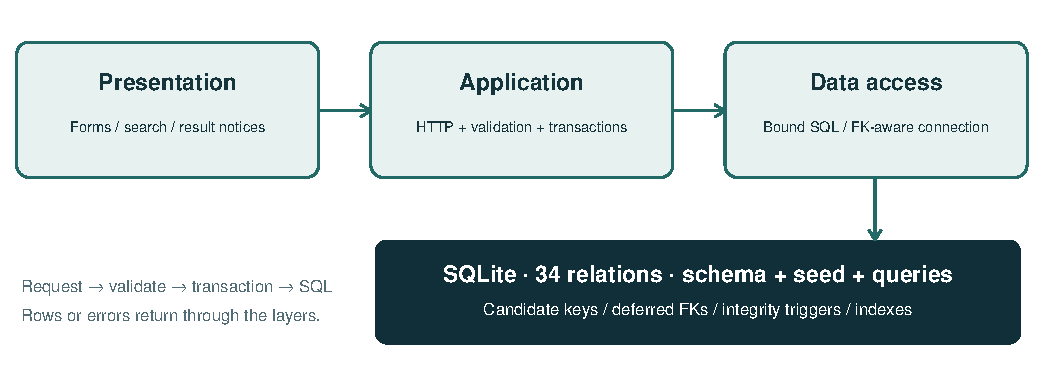
\includegraphics[width=\columnwidth]{architecture.pdf}
\caption{Implemented presentation, application/business and SQLite access layers. Source contains separate DDL, seed, queries and tests.}
\Description{Three application layers lead to a SQLite database with constraints and reproducible scripts.}
\end{figure}
\section{Operations and Observed Results}
\subsection{Creating and Populating the Database}
Separate scripts create 34 tables, integrity triggers and synthetic fixtures. Every relation is populated. The Id convention and preserved business key are illustrated by:
\begin{lstlisting}
CREATE TABLE Provider (
 Id INTEGER PRIMARY KEY AUTOINCREMENT,
 RegistrationJurisdiction TEXT NOT NULL,
 BusinessRegistrationNumber TEXT NOT NULL,
 LegalName TEXT NOT NULL,
 CONSTRAINT UK_Provider_BusinessKey UNIQUE
 (RegistrationJurisdiction,
  BusinessRegistrationNumber)
);
\end{lstlisting}
The complete DDL additionally rejects blank text. Parameterized forms insert and update providers; deleting an unused provider succeeds, while deleting a seeded provider fails due to FK references. Multi-table activity changes commit atomically or roll back on failure. SQL script 08 reproduces INSERT, SELECT, UPDATE and DELETE without relying on the interface.
\subsection{SELECT: Journey, Metrics and Awards}
The journey query joins activities, outlets, providers, accounts, vehicles and optional replacement services. A verified direct account-link predicate retains the local account identities. Observed output contains three rows: SALE-001 at Dealer A and SVC-001 at Provider C use VIN ending 4352; RENT-001 at Provider B uses VIN ending 4353 and explicitly references SVC-001.

The metric query aggregates contributions at measurement grain:
\begin{lstlisting}
SELECT m.Id, m.MeasuredValue,
 COUNT(DISTINCT c.VehicleActivityId) AS N
FROM PerformanceMeasurement m
LEFT JOIN MeasurementContribution c
 ON c.PerformanceMeasurementId=m.Id
GROUP BY m.Id,m.MeasuredValue;
\end{lstlisting}
Observed value and contribution count are both 1. The award view derives an event beneficiary through the subject activity's outlet, while a period beneficiary is its assessed provider. It returns 100 CAD for Dealer A and 10 POINT for Provider C. Evidence from another provider never changes these beneficiaries. The integrity audit returns zero rows.
\section{Architecture and Demonstration Interface}
The UI provides searchable relation tables, record forms, FK selectors, edit/delete actions and four joined views. The HTTP adapter routes requests to validation/transaction logic and a parameterized SQLite DAL. Relation names are allowlisted, data is bound as parameters, and mutation requests require a session token. The server binds only to the local loopback address. This is a coursework demonstration, without production login or deployment.
\begin{figure}[h]
\centering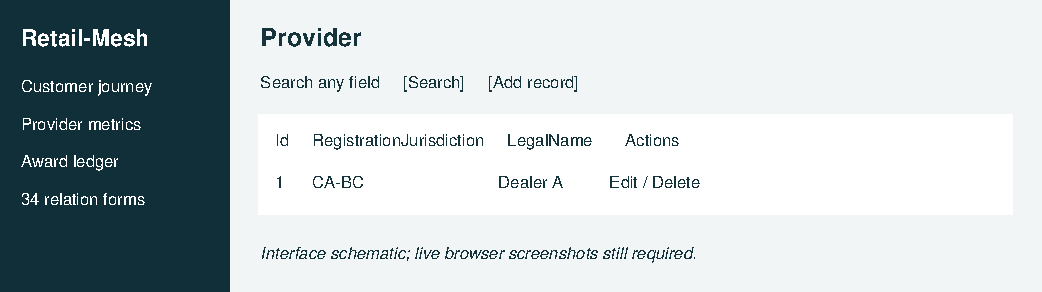
\includegraphics[width=\columnwidth]{ui-schematic.pdf}
\caption{Implemented controls shown schematically, not a browser screenshot. Required live operation screenshots must still be captured before submission.}
\Description{Sidebar, searchable provider table and edit and delete controls; schematic evidence only.}
\end{figure}
\section{Reproducibility and Critical Evaluation}
Python 3.10+ and its bundled SQLite suffice; the quickstart builds a fresh database from SQL and preserves subsequent edits. All 41 isolated database tests pass, including duplicate keys, invalid FKs, restricted deletion, rule overlap, atomic subtype creation, immutable evidence, award beneficiary consistency and minimum benefit participation. HTTP tests pass create/search/update/delete, reports, restricted deletion and CSRF checks. Observed outputs and test logs are included.

Browser execution was blocked by the environment's process/socket restrictions; visual CRUD verification and screenshots are pending. Arbitrary policy expressions are stored, not executed; synthetic qualifications are manually specified. Full authorization/enrollment eligibility and general multi-hop identity proof are reviewer responsibilities. AI drafted implementation, tests and this report~\cite{chatgpt}; automated checks are evidence, not a substitute for the team's critical evaluation or substantive contributions. Final author ordering, graduate-student-last compliance and human review must be confirmed before submission.
\begin{thebibliography}{1}
\bibitem{chatgpt} OpenAI. 2026. ChatGPT/Codex. AI-assisted relational mapping, implementation, tests and report drafting, November 3, 2026. Human evaluation pending.
\end{thebibliography}
\clearpage
\section*{Complete Relations and Constraints}
\fontsize{7}{8}\selectfont\raggedright
Every relation below also has \texttt{Id INTEGER PRIMARY KEY AUTOINCREMENT}. CK denotes mandatory UNIQUE business columns. A question mark marks a nullable column; all others are NOT NULL. All attributes ending in Id are FKs to the matching entity, except the exceptions below. References target Id; no deletion cascades. Full SQL and trigger conditions accompany this report.
\par\vspace{2.0pt}\noindent\textbf{ParentCompany}. \texttt{Registration\allowbreak{}Jurisdiction}, \texttt{Business\allowbreak{}Registration\allowbreak{}Number}, \texttt{Legal\allowbreak{}Name}.\par\noindent CK: \texttt{Registration\allowbreak{}Jurisdiction}, \texttt{Business\allowbreak{}Registration\allowbreak{}Number}.
\par\vspace{2.0pt}\noindent\textbf{ProviderAuthorization}. \texttt{Parent\allowbreak{}Company\allowbreak{}Id}, \texttt{Provider\allowbreak{}Id}, \texttt{Valid\allowbreak{}From}, \texttt{Valid\allowbreak{}To}?, \texttt{Authorization\allowbreak{}Status}.\par\noindent CK: \texttt{Parent\allowbreak{}Company\allowbreak{}Id}, \texttt{Provider\allowbreak{}Id}, \texttt{Valid\allowbreak{}From}.
\par\vspace{2.0pt}\noindent\textbf{VehicleModel}. \texttt{Manufacturer}, \texttt{Catalogue\allowbreak{}Namespace}, \texttt{Manufacturer\allowbreak{}Model\allowbreak{}Code}, \texttt{Model\allowbreak{}Year}, \texttt{Trim\allowbreak{}Code}, \texttt{Model\allowbreak{}Name}.\par\noindent CK: \texttt{Manufacturer}, \texttt{Catalogue\allowbreak{}Namespace}, \texttt{Manufacturer\allowbreak{}Model\allowbreak{}Code}, \texttt{Model\allowbreak{}Year}, \texttt{Trim\allowbreak{}Code}.
\par\vspace{2.0pt}\noindent\textbf{IncentiveProgram}. \texttt{Parent\allowbreak{}Company\allowbreak{}Id}, \texttt{Official\allowbreak{}Program\allowbreak{}Reference}, \texttt{Program\allowbreak{}Name}, \texttt{Active\allowbreak{}From}, \texttt{Active\allowbreak{}To}?, \texttt{Event\allowbreak{}Version\allowbreak{}Policy}, \texttt{Period\allowbreak{}Version\allowbreak{}Policy}.\par\noindent CK: \texttt{Parent\allowbreak{}Company\allowbreak{}Id}, \texttt{Official\allowbreak{}Program\allowbreak{}Reference}.
\par\vspace{2.0pt}\noindent\textbf{MetricDefinitionVersion}. \texttt{Parent\allowbreak{}Company\allowbreak{}Id}, \texttt{Official\allowbreak{}Metric\allowbreak{}Code}, \texttt{Effective\allowbreak{}From}, \texttt{Effective\allowbreak{}To}?, \texttt{Metric\allowbreak{}Name}, \texttt{Definition\allowbreak{}Expression}, \texttt{Unit\allowbreak{}Scheme}, \texttt{Unit\allowbreak{}Code}.\par\noindent CK: \texttt{Parent\allowbreak{}Company\allowbreak{}Id}, \texttt{Official\allowbreak{}Metric\allowbreak{}Code}, \texttt{Effective\allowbreak{}From}.
\par\vspace{2.0pt}\noindent\textbf{Provider}. \texttt{Registration\allowbreak{}Jurisdiction}, \texttt{Business\allowbreak{}Registration\allowbreak{}Number}, \texttt{Legal\allowbreak{}Name}.\par\noindent CK: \texttt{Registration\allowbreak{}Jurisdiction}, \texttt{Business\allowbreak{}Registration\allowbreak{}Number}.
\par\vspace{2.0pt}\noindent\textbf{CustomerAccount}. \texttt{Provider\allowbreak{}Id}, \texttt{Source\allowbreak{}Namespace}, \texttt{Existing\allowbreak{}Customer\allowbreak{}Reference}, \texttt{Display\allowbreak{}Name}, \texttt{Email}?, \texttt{Phone\allowbreak{}No}?.\par\noindent CK: \texttt{Provider\allowbreak{}Id}, \texttt{Source\allowbreak{}Namespace}, \texttt{Existing\allowbreak{}Customer\allowbreak{}Reference}.
\par\vspace{2.0pt}\noindent\textbf{Vehicle}. \texttt{VIN}, \texttt{Lifecycle\allowbreak{}Status}, \texttt{Vehicle\allowbreak{}Model\allowbreak{}Id}.\par\noindent CK: \texttt{VIN}.
\par\vspace{2.0pt}\noindent\textbf{ProgramEnrollment}. \texttt{Incentive\allowbreak{}Program\allowbreak{}Id}, \texttt{Provider\allowbreak{}Id}, \texttt{Valid\allowbreak{}From}, \texttt{Valid\allowbreak{}To}?, \texttt{Enrollment\allowbreak{}Status}.\par\noindent CK: \texttt{Incentive\allowbreak{}Program\allowbreak{}Id}, \texttt{Provider\allowbreak{}Id}, \texttt{Valid\allowbreak{}From}.
\par\vspace{2.0pt}\noindent\textbf{PerformanceMeasurement}. \texttt{Provider\allowbreak{}Id}, \texttt{Metric\allowbreak{}Definition\allowbreak{}Version\allowbreak{}Id}, \texttt{Period\allowbreak{}Start}, \texttt{Period\allowbreak{}End}, \texttt{Measured\allowbreak{}Value}, \texttt{Calculated\allowbreak{}At}.\par\noindent CK: \texttt{Provider\allowbreak{}Id}, \texttt{Metric\allowbreak{}Definition\allowbreak{}Version\allowbreak{}Id}, \texttt{Period\allowbreak{}Start}, \texttt{Period\allowbreak{}End}.
\par\vspace{2.0pt}\noindent\textbf{EventAwardComponent}. \texttt{Event\allowbreak{}Award\allowbreak{}Id}, \texttt{Reward\allowbreak{}Type}, \texttt{Unit\allowbreak{}Scheme}, \texttt{Unit\allowbreak{}Code}, \texttt{Benefit\allowbreak{}Value}, \texttt{Currency}?, \texttt{Valid\allowbreak{}From}, \texttt{Valid\allowbreak{}To}?.\par\noindent CK: \texttt{Event\allowbreak{}Award\allowbreak{}Id}, \texttt{Reward\allowbreak{}Type}, \texttt{Unit\allowbreak{}Scheme}, \texttt{Unit\allowbreak{}Code}. Other UQ: (\texttt{Id},\texttt{Event\allowbreak{}Award\allowbreak{}Id}).
\par\vspace{2.0pt}\noindent\textbf{Outlet}. \texttt{Provider\allowbreak{}Id}, \texttt{Existing\allowbreak{}Outlet\allowbreak{}Reference}, \texttt{Outlet\allowbreak{}Name}, \texttt{Address}.\par\noindent CK: \texttt{Provider\allowbreak{}Id}, \texttt{Existing\allowbreak{}Outlet\allowbreak{}Reference}.
\par\vspace{2.0pt}\noindent\textbf{CustomerIdentityLink}. \texttt{Account\allowbreak{}AId}, \texttt{Account\allowbreak{}BId}, \texttt{Verification\allowbreak{}Status}, \texttt{Verification\allowbreak{}Method}, \texttt{Verified\allowbreak{}At}?, \texttt{Revoked\allowbreak{}At}?, \texttt{Evidence\allowbreak{}Reference}.\par\noindent CK: \texttt{Account\allowbreak{}AId}, \texttt{Account\allowbreak{}BId}. FK exceptions: \texttt{Account\allowbreak{}AId}$\to$\texttt{Customer\allowbreak{}Account}; \texttt{Account\allowbreak{}BId}$\to$\texttt{Customer\allowbreak{}Account}.
\par\vspace{2.0pt}\noindent\textbf{VehicleActivity}. \texttt{Issuing\allowbreak{}Outlet\allowbreak{}Id}, \texttt{Source\allowbreak{}Namespace}, \texttt{Activity\allowbreak{}Kind}, \texttt{Official\allowbreak{}Activity\allowbreak{}Reference}, \texttt{Activity\allowbreak{}Status}, \texttt{Started\allowbreak{}At}, \texttt{Ended\allowbreak{}At}?, \texttt{Recorded\allowbreak{}At}, \texttt{Customer\allowbreak{}Account\allowbreak{}Id}, \texttt{Vehicle\allowbreak{}Id}, \texttt{Sale\allowbreak{}Id}?, \texttt{Rental\allowbreak{}Id}?, \texttt{Service\allowbreak{}Id}?.\par\noindent CK: \texttt{Issuing\allowbreak{}Outlet\allowbreak{}Id}, \texttt{Source\allowbreak{}Namespace}, \texttt{Activity\allowbreak{}Kind}, \texttt{Official\allowbreak{}Activity\allowbreak{}Reference}. FK exceptions: \texttt{Issuing\allowbreak{}Outlet\allowbreak{}Id}$\to$\texttt{Outlet}. Other UQ: (\texttt{Id},\texttt{Sale\allowbreak{}Id}); (\texttt{Id},\texttt{Rental\allowbreak{}Id}); (\texttt{Id},\texttt{Service\allowbreak{}Id}).
\par\vspace{2.0pt}\noindent\textbf{IncentiveRule}. \texttt{Incentive\allowbreak{}Program\allowbreak{}Id}, \texttt{Official\allowbreak{}Rule\allowbreak{}Code}, \texttt{Rule\allowbreak{}Name}, \texttt{Assessment\allowbreak{}Basis}.\par\noindent CK: \texttt{Incentive\allowbreak{}Program\allowbreak{}Id}, \texttt{Official\allowbreak{}Rule\allowbreak{}Code}.
\par\vspace{2.0pt}\noindent\textbf{EventEvaluation}. \texttt{Vehicle\allowbreak{}Activity\allowbreak{}Id}, \texttt{Rule\allowbreak{}Version\allowbreak{}Id}, \texttt{Result}, \texttt{Reason}, \texttt{Qualification\allowbreak{}Date}, \texttt{Evaluated\allowbreak{}At}, \texttt{Decision\allowbreak{}Evidence\allowbreak{}Reference}.\par\noindent CK: \texttt{Vehicle\allowbreak{}Activity\allowbreak{}Id}, \texttt{Rule\allowbreak{}Version\allowbreak{}Id}.
\par\vspace{2.0pt}\noindent\textbf{EventAward}. \texttt{Vehicle\allowbreak{}Activity\allowbreak{}Id}, \texttt{Incentive\allowbreak{}Rule\allowbreak{}Id}, \texttt{Award\allowbreak{}Status}, \texttt{Issued\allowbreak{}At}, \texttt{Accepted\allowbreak{}Evaluation\allowbreak{}Id}, \texttt{First\allowbreak{}Component\allowbreak{}Id}.\par\noindent CK: \texttt{Vehicle\allowbreak{}Activity\allowbreak{}Id}, \texttt{Incentive\allowbreak{}Rule\allowbreak{}Id}. FK exceptions: \texttt{Accepted\allowbreak{}Evaluation\allowbreak{}Id}$\to$\texttt{Event\allowbreak{}Evaluation}; \texttt{First\allowbreak{}Component\allowbreak{}Id}$\to$\texttt{Event\allowbreak{}Award\allowbreak{}Component}. Other UQ: (\texttt{Accepted\allowbreak{}Evaluation\allowbreak{}Id}).
\par\vspace{2.0pt}\noindent\textbf{Capability}. \texttt{Existing\allowbreak{}Capability\allowbreak{}Designation}, \texttt{Description}.\par\noindent CK: \texttt{Existing\allowbreak{}Capability\allowbreak{}Designation}.
\par\vspace{2.0pt}\noindent\textbf{CapabilityAuthorization}. \texttt{Provider\allowbreak{}Authorization\allowbreak{}Id}, \texttt{Outlet\allowbreak{}Id}, \texttt{Capability\allowbreak{}Id}, \texttt{Valid\allowbreak{}From}, \texttt{Valid\allowbreak{}To}?, \texttt{Authorization\allowbreak{}Status}.\par\noindent CK: \texttt{Provider\allowbreak{}Authorization\allowbreak{}Id}, \texttt{Outlet\allowbreak{}Id}, \texttt{Capability\allowbreak{}Id}, \texttt{Valid\allowbreak{}From}.
\par\vspace{2.0pt}\noindent\textbf{RuleVersion}. \texttt{Incentive\allowbreak{}Rule\allowbreak{}Id}, \texttt{Effective\allowbreak{}From}, \texttt{Effective\allowbreak{}To}?, \texttt{Condition\allowbreak{}Expression}, \texttt{Reward\allowbreak{}Specification}.\par\noindent CK: \texttt{Incentive\allowbreak{}Rule\allowbreak{}Id}, \texttt{Effective\allowbreak{}From}.
\par\vspace{2.0pt}\noindent\textbf{PeriodEvaluation}. \texttt{Provider\allowbreak{}Id}, \texttt{Rule\allowbreak{}Version\allowbreak{}Id}, \texttt{Period\allowbreak{}Start}, \texttt{Period\allowbreak{}End}, \texttt{Result}, \texttt{Reason}, \texttt{Qualification\allowbreak{}Date}, \texttt{Evaluated\allowbreak{}At}, \texttt{Decision\allowbreak{}Evidence\allowbreak{}Reference}.\par\noindent CK: \texttt{Provider\allowbreak{}Id}, \texttt{Rule\allowbreak{}Version\allowbreak{}Id}, \texttt{Period\allowbreak{}Start}, \texttt{Period\allowbreak{}End}.
\par\vspace{2.0pt}\noindent\textbf{PeriodAward}. \texttt{Provider\allowbreak{}Id}, \texttt{Incentive\allowbreak{}Rule\allowbreak{}Id}, \texttt{Period\allowbreak{}Start}, \texttt{Period\allowbreak{}End}, \texttt{Award\allowbreak{}Status}, \texttt{Issued\allowbreak{}At}, \texttt{Accepted\allowbreak{}Evaluation\allowbreak{}Id}, \texttt{First\allowbreak{}Component\allowbreak{}Id}.\par\noindent CK: \texttt{Provider\allowbreak{}Id}, \texttt{Incentive\allowbreak{}Rule\allowbreak{}Id}, \texttt{Period\allowbreak{}Start}, \texttt{Period\allowbreak{}End}. FK exceptions: \texttt{Accepted\allowbreak{}Evaluation\allowbreak{}Id}$\to$\texttt{Period\allowbreak{}Evaluation}; \texttt{First\allowbreak{}Component\allowbreak{}Id}$\to$\texttt{Period\allowbreak{}Award\allowbreak{}Component}. Other UQ: (\texttt{Accepted\allowbreak{}Evaluation\allowbreak{}Id}).
\par\vspace{2.0pt}\noindent\textbf{Rental}. \texttt{Vehicle\allowbreak{}Activity\allowbreak{}Id}, \texttt{Rental\allowbreak{}Charge}, \texttt{Currency}, \texttt{Returned\allowbreak{}At}?, \texttt{Replacement\allowbreak{}For\allowbreak{}Service\allowbreak{}Id}?, \texttt{Replacement\allowbreak{}Purpose}?.\par\noindent CK: \texttt{Vehicle\allowbreak{}Activity\allowbreak{}Id}. FK exceptions: \texttt{Replacement\allowbreak{}For\allowbreak{}Service\allowbreak{}Id}$\to$\texttt{Service}. Other UQ: (\texttt{Id},\texttt{Vehicle\allowbreak{}Activity\allowbreak{}Id}).
\par\vspace{2.0pt}\noindent\textbf{Sale}. \texttt{Vehicle\allowbreak{}Activity\allowbreak{}Id}, \texttt{Sale\allowbreak{}Price}, \texttt{Currency}, \texttt{Completed\allowbreak{}At}.\par\noindent CK: \texttt{Vehicle\allowbreak{}Activity\allowbreak{}Id}. Other UQ: (\texttt{Id},\texttt{Vehicle\allowbreak{}Activity\allowbreak{}Id}).
\par\vspace{2.0pt}\noindent\textbf{Service}. \texttt{Vehicle\allowbreak{}Activity\allowbreak{}Id}, \texttt{Service\allowbreak{}Type}, \texttt{Outcome}, \texttt{Completed\allowbreak{}At}.\par\noindent CK: \texttt{Vehicle\allowbreak{}Activity\allowbreak{}Id}. Other UQ: (\texttt{Id},\texttt{Vehicle\allowbreak{}Activity\allowbreak{}Id}).
\par\vspace{2.0pt}\noindent\textbf{PeriodAwardComponent}. \texttt{Period\allowbreak{}Award\allowbreak{}Id}, \texttt{Reward\allowbreak{}Type}, \texttt{Unit\allowbreak{}Scheme}, \texttt{Unit\allowbreak{}Code}, \texttt{Benefit\allowbreak{}Value}, \texttt{Currency}?, \texttt{Valid\allowbreak{}From}, \texttt{Valid\allowbreak{}To}?.\par\noindent CK: \texttt{Period\allowbreak{}Award\allowbreak{}Id}, \texttt{Reward\allowbreak{}Type}, \texttt{Unit\allowbreak{}Scheme}, \texttt{Unit\allowbreak{}Code}. Other UQ: (\texttt{Id},\texttt{Period\allowbreak{}Award\allowbreak{}Id}).
\par\vspace{2.0pt}\noindent\textbf{MeasurementContribution}. \texttt{Performance\allowbreak{}Measurement\allowbreak{}Id}, \texttt{Vehicle\allowbreak{}Activity\allowbreak{}Id}, \texttt{Contribution\allowbreak{}Role}.\par\noindent CK: \texttt{Performance\allowbreak{}Measurement\allowbreak{}Id}, \texttt{Vehicle\allowbreak{}Activity\allowbreak{}Id}.
\par\vspace{2.0pt}\noindent\textbf{RuleMetric}. \texttt{Rule\allowbreak{}Version\allowbreak{}Id}, \texttt{Metric\allowbreak{}Definition\allowbreak{}Version\allowbreak{}Id}, \texttt{Metric\allowbreak{}Role}.\par\noindent CK: \texttt{Rule\allowbreak{}Version\allowbreak{}Id}, \texttt{Metric\allowbreak{}Definition\allowbreak{}Version\allowbreak{}Id}.
\par\vspace{2.0pt}\noindent\textbf{EventEvaluationMeasurement}. \texttt{Event\allowbreak{}Evaluation\allowbreak{}Id}, \texttt{Performance\allowbreak{}Measurement\allowbreak{}Id}, \texttt{Evidence\allowbreak{}Role}.\par\noindent CK: \texttt{Event\allowbreak{}Evaluation\allowbreak{}Id}, \texttt{Performance\allowbreak{}Measurement\allowbreak{}Id}.
\par\vspace{2.0pt}\noindent\textbf{EventEvaluationActivity}. \texttt{Event\allowbreak{}Evaluation\allowbreak{}Id}, \texttt{Vehicle\allowbreak{}Activity\allowbreak{}Id}, \texttt{Evidence\allowbreak{}Role}.\par\noindent CK: \texttt{Event\allowbreak{}Evaluation\allowbreak{}Id}, \texttt{Vehicle\allowbreak{}Activity\allowbreak{}Id}.
\par\vspace{2.0pt}\noindent\textbf{EventEvaluationIdentity}. \texttt{Event\allowbreak{}Evaluation\allowbreak{}Id}, \texttt{Customer\allowbreak{}Identity\allowbreak{}Link\allowbreak{}Id}, \texttt{Verification\allowbreak{}Outcome\allowbreak{}Used}, \texttt{Verified\allowbreak{}At\allowbreak{}Used}, \texttt{Evidence\allowbreak{}Reference\allowbreak{}Used}.\par\noindent CK: \texttt{Event\allowbreak{}Evaluation\allowbreak{}Id}, \texttt{Customer\allowbreak{}Identity\allowbreak{}Link\allowbreak{}Id}.
\par\vspace{2.0pt}\noindent\textbf{PeriodEvaluationMeasurement}. \texttt{Period\allowbreak{}Evaluation\allowbreak{}Id}, \texttt{Performance\allowbreak{}Measurement\allowbreak{}Id}, \texttt{Evidence\allowbreak{}Role}.\par\noindent CK: \texttt{Period\allowbreak{}Evaluation\allowbreak{}Id}, \texttt{Performance\allowbreak{}Measurement\allowbreak{}Id}.
\par\vspace{2.0pt}\noindent\textbf{PeriodEvaluationActivity}. \texttt{Period\allowbreak{}Evaluation\allowbreak{}Id}, \texttt{Vehicle\allowbreak{}Activity\allowbreak{}Id}, \texttt{Evidence\allowbreak{}Role}.\par\noindent CK: \texttt{Period\allowbreak{}Evaluation\allowbreak{}Id}, \texttt{Vehicle\allowbreak{}Activity\allowbreak{}Id}.
\par\vspace{2.0pt}\noindent\textbf{PeriodEvaluationIdentity}. \texttt{Period\allowbreak{}Evaluation\allowbreak{}Id}, \texttt{Customer\allowbreak{}Identity\allowbreak{}Link\allowbreak{}Id}, \texttt{Verification\allowbreak{}Outcome\allowbreak{}Used}, \texttt{Verified\allowbreak{}At\allowbreak{}Used}, \texttt{Evidence\allowbreak{}Reference\allowbreak{}Used}.\par\noindent CK: \texttt{Period\allowbreak{}Evaluation\allowbreak{}Id}, \texttt{Customer\allowbreak{}Identity\allowbreak{}Link\allowbreak{}Id}.
\par\vspace{4pt}\textbf{Shared domain and cross-row constraints.} Business CK values are immutable after insertion. Dates use YYYY-MM-DD, timestamps use canonical UTC. Valid/effective/active, activity and period end values must exceed their starts; NULL end is unbounded. Prices/charges/benefits are nonnegative; currencies are three uppercase letters when supplied. VIN is 17 permitted uppercase characters. Identity pairs have AccountAId $<$ AccountBId; Verified requires VerifiedAt and no revocation. Activity kind is Sale, Rental or Service; exactly one matching owned subtype is mandatory through bidirectional deferred composite FKs. Rental replacement service and purpose must be jointly present or absent. AssessmentBasis is Event or Period; results are Qualified or Rejected; award status is Issued or Cancelled. AcceptedEvaluationId is unique, qualified, and matches subject, rule and period; FirstComponentId forces at least one owned benefit. Overlapping authorization, enrollment and definition/version intervals are rejected. Evaluations and cited evidence sources are immutable. Evidence is append-only until acceptance, then frozen; identity snapshots must match a currently verified assertion. Program/authorization eligibility is retained for reviewer validation, not automatically certified.

\end{document}
